% Note that if you want something in single space you can go back and
% forth between single space and normal space by the use of \ssp and
% \nsp.  If you want doublespacing you can use \dsp.  \nsp is normally
% 1.5 spacing unless you use the doublespace option (or savepaper
% option)
%
%(FORMAT) Usually you *don't* want to mess with the spacing for your
%(FORMAT) final version.  If you think/know that the thesis template
%(FORMAT) and/or thesis style file is incorrect/incomplete, PLEASE
%(FORMAT) contact the maintainer.  THANK YOU!!!

\chapter{INTRODUCTION}
\label{chap:intro}
% By labeling the chapter, I can refer to it later using the
% label. (\ref{chap:intro}, \pageref{chap:intro}) Latex will take care
% of the numbering.

In the study of dynamical systems a central problem is how to derive models 
from measured data to facilitate the prediction of future states. Many 
approaches and techniques exist in the literature, from deriving sets of 
governing equations via application of the simple physical principles to 
the statistically meaningful Principal Component Analysis and other modal 
decompositions. The main goal of many of these methods is to come up with 
a generalized framework so that the dynamics can be extracted from the data
for the sake of control and prediction. While there are genuine advantages
to the more concrete and scientifically-sound methods of deriving models 
from first principles, it is often very difficult if not outright untenable.

As such, data-driven methods have rapidly become very useful approaches for 
coming up with rough and ready models. 

Say more once you've thought of it.

\section{What is E-DMD?}
As it says on the tin, we seek a predictive model for a time series $\bracks{
\boldsymbol{y}_j}_{j=1}^{N^T+1}$, which are the measurements of a uniformly 
sampled unknown dynamical system of the form
$$\dd{\boldsymbol{y}}{t} = f\parens{\boldsymbol{y}(t)},\quad \boldsymbol{y}(0) 
= \boldsymbol{x} \in \mathcal{M} \subseteq \R^{N_s}$$
As established in the introduction, there is an old and venerable literature 
dedicated to deriving system using classical methods. What this literature will 
admit is that such a process is not trivial and even difficult or impossible to 
do in practice; particularly for nonlinear phenomena worth investigating. We 
want something that is more easily generalized and algorithmic.

One method that can be leveraged for this is via the Koopman Operator 
$\mathcal{K}$. If we denote $\boldsymbol{\varphi}(t;\boldsymbol{x}) =
\boldsymbol{y}(t)$ to be the flow map affiliated with the initial condition 
$\boldsymbol{x}$ and denote $g: \mathcal{M} \to \C$ to be a square integrable 
observable of the system then, according to \cite{koopman}, there exists a 
linear representation of the flow map given by $\mathcal{K}$;
$$\mathcal{K}^t g(\boldsymbol{x}) = g(\boldsymbol{\varphi}(t; \boldsymbol{x}))
,$$
which means that $\mathcal{K}$ is a linear time-advancement operator of the 
dynamics. This might seem like it trivializes the problem, given that we now 
have a linear system, but it does not. The Koopman operator is an 
\emph{infinite} dimensional operator, so we've traded a potentially nonlinear 
problem for an infinite dimensional linear one.

In order to actually use this new representation, it suffices to find the 
eigenvalues $\bracks{\lambda_\ell}$, and their affiliated eigenfunctions 
$\bracks{\boldsymbol{\phi}_\ell}$, of the Koopman Operator such that
$$\mathcal{K}^t\boldsymbol{\phi}_\ell = \exp(t\lambda_\ell)\boldsymbol{\phi}
_\ell \implies g(\boldsymbol{x}) = \sum_{\ell \in \N} c_\ell \boldsymbol{\phi}_
\ell(\boldsymbol{x}),$$
where we can essentially construct a modal decomposition of $g$. From here 
advancing the dynamics to time $t$ is equivalent to writing
$$\mathcal{K}^{t} g(\boldsymbol{x}) = \sum_{\ell \in \N} a_\ell \boldsymbol{
  \phi}_\ell (\boldsymbol{\varphi}(t,\boldsymbol{x}))$$
The most useful property of this framing is that we have a global linearization 
of the flow, with a major caveat: Generally, finding these eigenvalues and 
eigenfunctions is impossible. This led to the development of the already 
mentioned and much much lauded Dynamic Mode Decomposition (DMD) and it's 
extensions, which seeks to numerically approximate a finite number of these 
modes. We'll focus on the particular extension that \cite{lago} implements: 
Extended DMD (E-DMD) \cite{williams}. With E-DMD, we suppose that 
$$g(\boldsymbol{x}) = \sum_{\ell = 1}^{N_O} a_\ell \boldsymbol{\psi}_\ell
(\boldsymbol{x})$$
which is to say that the observable $g$ exists in a finite dimensional subspace 
of $L^2(\mathcal{M})$, applying the Koopman operator implies that
\begin{align*} 
    \mathcal{K}^{\delta t} g(\boldsymbol{x}) &= \sum_{\ell = 1}^{N_O} a_\ell 
    \boldsymbol{\phi}_\ell
    (\boldsymbol{\varphi}(\delta t,\boldsymbol{x})) \\
    &= \sum_{\ell = 1}^{N_O} \boldsymbol{\phi}_\ell (\boldsymbol{x})
    (\boldsymbol{K}_O^T
    \boldsymbol{a})_\ell + r(\boldsymbol{x};\boldsymbol{K}_O)
\end{align*}
for discrete time step $\delta t$. $K_O$ is the $N_O\times N_O$ matrix that 
minimizes
$$\boldsymbol{K}_O = \underset{K}{\text{argmin}}\norm{\Psi_+ - K\Psi_-}_F^2$$
and $r(\boldsymbol{x}, \boldsymbol{K}_O)$ is a residual that represents the 
total error due to DMD. If the ansatz that $g$ lives in a finite space holds, 
then $r$ is identically 0. We define $\Psi_\pm$ to be
$$\Psi_- = \parens{\Psi_1\ \Psi_2\ \cdots \Psi_{N_T}},\quad \Psi_+ = \parens{
  \Psi_2\ \Psi_3\ \cdots \Psi_{N_T+1}}$$
where $\bracks{\Psi_j}$ is an observable of the time series of interest 
$\bracks{\boldsymbol{y}_j}$. What the expression for $\boldsymbol{K}_O$ tells 
us is that, we are trying to find a one-step mapping from each data point
to the next. Practically speaking, $\boldsymbol{K}_O$ is found
%$\boldsymbol{K}_O$ approximates $\mathcal{K}$ for a one-step mapping and is found 
using an SVD, with which we can write
$$\Psi_- = U\Sigma W^{\dagger} \implies \boldsymbol{K}_O = \Psi_+W\Sigma^{-P}
U^{\dagger}$$
where $-P$ denotes the Moore-Penrose pseudo-inverse and $\dagger$ denotes the 
conjugate transpose. This gives us an expression for $r$ in terms of the 
observables $\Psi$:
$$E_r(\boldsymbol{K}_O) = \norm{\Psi_+(I - WW^\dagger)}_F$$
% and we can find with an 
%explicit expression it using an SVD on $\Psi_-$. 
Finding the eigenvalues, eigenfunctions, and Koopman modes comes down to an 
eigen-decomposition, from which the dynamics can be approximated as 
$$y(t;\boldsymbol{x}) \approx V\exp(t\Lambda)V^{-1}\boldsymbol{\Psi}
(\boldsymbol{x})$$
where $\boldsymbol{K}_O = VTV^{-1}$, $\Lambda_{\ell\ell} = \ln(T_{\ell\ell})/
\delta t$ is a diagonal matrix and $\boldsymbol{\Psi}$ is the representation 
of the initial condition in terms of the observables. 

\section{What are Neural Networks?}

Before we move on, a brief digression on Neural Networks (NNs) is appropriate. Ever since
scientists discovered the relatively simple interaction between neurons and axons in 
the human brain, they have been enamored with the ability to create a learning computer 
with the similar ability to become more adept at a task with training and practice. 
In the same way that art imitates life, the most straight-forward attempts have been 
to construct artificial neural networks that pantomime the biological ones that we carry 
around in our heads; and while these pale imitations have not been developed to rival the 
human brain, they have led to some major achievements in automation. In much the same 
way that a person is ``trained'' to perform a task by repeating it with feedback and 
adjusting their performance as they go, an artificial NN uses data, a loss function, and 
an optimization algorithm to change the state of the NN to one which can better accomplish 
the task. The loss function and optimizer are to the feedback and behavioral adjustment 
what the data is to the experience. 

The oldest known example 
of NNs were the perceptrons of the 1950s, which could perform binary classifications of 
linearly separable data. Multilayer versions of this simple architecture allowed for 
classification of larger set of classes, but the researcher of the time arrived at the 
limits of their computing environments rather quickly and a brief dark age in the study 
and application of neural networks ensued. Interest was renewed in the 1980s when many 
of the hardware limitations of previous decades were ameliorated and new algorithms for 
optimizing had been pioneered.

In modern mathematical study and application, the question of function representation is
an ever-present one; specifically with respect to approximating quantities that can be 
given via series. While truncations and use of the likes of fourier series are useful and 
effective in some narrow applications, one means of representation that has shown much 
promise in recent years due to the greater availability of computing power is through 
the use of Neural Networks (NNs). In 1989, \cite{hornik} showed that, with some appropriate
parameters, a NN can be used to approximate any continuous function from one vector space 
to another to any arbitrary precision required. 

From this we can consider ML as a tool of regression. Say we have a set of training data
$d_{tr} = \bracks{(x_j, y_j)}_{j=1}^{N_{tr}}$ and we believe that there is some function
$f(x)$ such that 
$$y_j = f(x_j) + \vep_j,$$
where $\vep_j$ is assumed to be a sample drawn from $\mathcal{N}(0, \bar{\sigma}^2)$. 
Generally $f$ is not known; so we must, using the training data, build an estimator 
$f_e(x; d_{tr})$ and measure the performance of the estimator by examining the quantity
$$\mathbb{E}_{d_{tr}}\sqbracks{\parens{f(x) + \vep - f_e(x;d_{tr})}^2} = 
\text{bias}_{d_{tr}}^2 + \mathbb{V}(f_e) + \bar{\sigma}^2$$
where 
$$\text{bias}_{d_{tr}} = \mathbb{E}_{d_{tr}}\sqbracks{f_e} - f(x)$$
and 
$$\mathbb{V}(f_e) = \mathbb{E}_{d_{tr}}\sqbracks{\parens{\mathbb{E}_{d_{tr}}\sqbracks{f_e} - f_e(x; d_{tr})}^2}$$ 
With this framing, ML methods can be cast as attempts to find an estimator relative to
a given training that balances the competing dilemmas of being too biased or allowing too
much variance. From the point of view of non-parametric statistics, we would need to utilize 
other techniques\cite{hollander} to determine the bias and variance of any given estimator. For our purposes, 
we will instead consider how metrics from information theory can be used to assess the change in 
information as data is fed through a NN and a model is trained.

\section{DLDMD and it's limitations}

The key innovation of 
\cite{lago} is to use a neural network to come up with the collection of 
observables on $\bracks{\boldsymbol{y}_j}$ that allow for the best prediction 
of future system states. This is implemented by defining an encoder 
$\mathcal{E}: N_S \to N_O$ and decoder $\mathcal{D}: N_O \to N_S$ composed of 
Dense layers such that 
$$(\mathcal{D}\circ\mathcal{E})(\boldsymbol{x}) = \boldsymbol{x}$$
We choose $N_O \geq N_S$ and an appropriate loss function so that 
$\mathcal{E}$ and $\mathcal{D}$ give a richer space of observables, called the 
latent space, for EDMD to use when advancing the dynamics. The implementation 
of NNs for this purpose requires a method of tuning to allow $\mathcal{E}$ and 
$\mathcal{D}$ to learn the best representations possible. As such, a loss 
function that correctly identifies and prioritizes the desired properties is 
a necessary condition for the DLDMD to function as needed. A natural choice
considering these constraints is given by
\begin{equation}
    \mathcal{L} = \alpha_1 \mathcal{L}_{\text{recon}} + \alpha_2 \mathcal{L}
    _{\text{dmd}} + \alpha_3 \mathcal{L}_{\text{pred}} +\alpha_4 
    \norm{\boldsymbol{W}_g}_2^2 \label{eqn:loss function} 
\end{equation}
where 
\begin{align}
    \mathcal{L}_{\text{recon}} &= \frac{1}{N_T + 1}\sum_{j=1}^{N_T+1}\norm{\boldsymbol{y}_j - 
    (\mathcal{D}\circ\mathcal{E})(\boldsymbol{y}_j)}_2, \\
    \mathcal{L}_{\text{dmd}} &= E_r(\boldsymbol{K}_O), \\
    \mathcal{L}_{\text{pred}} &= \frac{1}{N_T}\sum_{j=1}^{N_T}\norm{\boldsymbol{y}_{j+1} - 
    \mathcal{D}\parens{VT^j V^{-1}\mathcal{E}(x)}}_2, \label{eqn:blah}
\end{align}
Each component guides the machine to a particular outcome: 
\begin{enumerate}
    \item $\mathcal{L}_{\text{recon}}$ is the Mean Squared Error (MSE) of each time step
    with respect to the reconstruction from the composition of $\mathcal{E}$ and $\mathcal{D}$. 
    This component ensures that, under training, the network effectively acts as a near identity 
    transformation for data that is fed into it. This quality allows the DMD advanced trajectories 
    to be recovered from the higher dimensional latent space back to the original dimension of 
    the data.
    
    \item $\mathcal{L}_{\text{DMD}}$ is the error associated with DMD. Consequently, this 
    component is the one that is most responsible for finding the optimal set of observables for DMD.
    $\mathcal{E}$ immerses the data into a higher dimensional latent space, in effect acting as our 
    set of observable; minimizing this gives us greater flexibility in the latent space.
    
    \item $\mathcal{L}_{\text{pred}}$ is the (MSE) for each forward time prediction due to DMD and 
    immersion/submersion due to $\mathcal{E}/\mathcal{D}$. In addition to balancing the last conditions, 
    this condition ensures that the DMD step in the latent dimension is consistent with the next time-step from 
    the time series after encoding, advancing, and decoding.  
    
    \item $\boldsymbol{W}_g$ is the vectorized quantity that represents all weights in both $\mathcal{E}$
    and $\mathcal{D}$. This is really only a regularization condition to keep the coefficients of the 
    weight matrices from blowing up in value as the model trains, which can be a 
    concern for ML models.
    
    \item $\alpha_1,\ \alpha_2,\ \alpha_3,$ and $\alpha_4$ are 4 positive constants that allow us to assign a 
    weighting to each component of the loss. This allows the loss function to be dynamically weighted to 
    prioritize some conditions over others. In \cite{lago}, $\alpha_1 = \alpha_2 = \alpha_3 = 1$ and 
    $\alpha_4 < 10^{-10}$.
\end{enumerate}

The marriage of E-DMD with Dense NNs and some meaningful choices of loss function as 
an innovation was made by \cite{lago, brunton, lusch}, and has proved to be quite a 
robust method for learning dynamics from data. In researching this thesis, many attempts 
were made to test the limits of DLDMD. \cite{lago} was primarily interested in recreating 
the phase space behavior of a handful of well known nonlinear oscillators such as the 
nonlinear harmonic oscillator, the Duffing oscillator, and the Van der Pol oscillator. 
Additionally, chaotic systems like Lorenz 63 and the R\"{o}ssler system were examined but 
chaos proved to be quite a challenge for the algorithm to overcome. A study into the addition
of gaussian noise led to the discovery of the machine being quite robust to data due to the 
characteristics of it's loss function and additional noise mitigation was accomplished by 
implementing convolutional layers instead of traditional dense layers.

\section{Statement of Dilemma}
Having estabilshed DLDMD and having discussed testing it's limitations via training 
new models and \emph{visually} qualifying each run as a success or failure, a question is 
begged: Can we, in an empirical and quantitative fashion, determine whether good training 
is taking place or otherwise deduce whether our model is well-posed given the 
hyperparameters?
A machine learning model that must learn how to accomplish even a simple task can take 
quite a long time and plenty of computing resources to complete it's training and only then 
can the results be checked to determine whether productive training was taking place as 
opposed to the optimizer becoming stuck in a local minimum or there being no global 
minimum at all.

How can this be quantified? A useful starting point would be to examine the weights of
the matrices that make up the layers of a model. For Dense layers, passing a vector of 
data $\boldsymbol{x} \in \R^{d}$ through a layer $L$ can be written as 
$$L(\boldsymbol{x}; A, \sigma, b) = \sigma(A\boldsymbol{x} + b)$$
for some matrix $A \in \R^{D\times d}$, vector $b \in \R^{D}$ and (typically nonlinear)
activation function $\sigma: \R^D \to \R^D$. For a given layer, $\sigma$ is a fixed 
hyperparameter of the machine, but both $A$ and $b$ have entries that are tuned by the 
optimizer as training takes places. Training takes place on a per epoch basis for most 
models, so considering the configuration of these matrices epoch to epoch can help us 
determine whether they are converging to a set of elements that accomplish the desired 
task or not. The next state for each layer is dependent on the previous, so a reasonable 
framing would be as one of a discrete dynamical system of the form
$$Q_{n+1} = P(Q_n) \quad (\text{Come up with better symbols later})$$
where $P$ is the training procedure and $Q_n$ represents the configuration of the network's
weights at each epoch $n$. Typically, the initial state $Q_0$ is ``random'' in the sense 
that the weights are selected from a probability distribution. In the interest of examining 
convergences, one might consider the following limit 
$$\lim \norm{Q_{n+1} - Q_n}_2$$
for some $L^2$ norm on the space that $Q_n$ inhabits. While this ``one-step'' Cauchy 
convergence will tell us whether the machine is approaching a particular configuration
point-wise, this might not actually tell us much of anything else. The changes between 
epochs is, in some sense, stochastic due to not knowing how the optimizer will update $Q$
between epochs. As such, we propose a more statistical approach wherein we examine how the
information content is changing from epoch to epoch. By the noted stochastic nature of the 
evolution, we consider the entries of $A$ and $b$ for each layer to be drawn from a continuous 
probability distribution $X$ and examine how it changes epoch to epoch. 


\chapter{KULLBACK-LEIBLER DIVERGENCE}
\label{chap:KLD}
In the field of information theory, it is often useful to frame information as being 
represented by a random variable and the values it can take on. For example, consider 
a normally distributed random variable $X \sim \mathcal{N}(\mu, \sigma^2)$ where $\mu$ is the 
mean or expected value $\mathbb{E}[X]$ of $X$ and $\sigma^2$ is the variance 
$\mathbb{V}[X]$ of $X$. This is one of the most well understood probability distributions
due to countless years of study into its properties, as such we know that if we were to 
draw a sample for $X$ that we're much more likely to get something close to $\mu$
than we are to get something far away from $\mu$. For example; if $\mu = 0$ and 
$\sigma^2 = 1$, then upon drawing a sample the value 1 is more likely to appear
than -37. The level of certainty of the outcome of the draw begs the question of 
how that certainty can be quantified and conversely, we could instead consider the 
uncertainty of any given probability distribution. A measure of the uncertainty was 
proposed in 1948 and this measure is known as \emph{informational entropy} \cite{shannon}
or, simply, entropy. For a
continuous distribution with density function $f(x)$, the entropy is given by 
\begin{equation}
    h[f] = \mathbb{E}\sqbracks{-\log(f(x))} = -\int_X f(x)\log(f(x))\ dx    
\end{equation}
For the normall distributed $X$ defined above, we have that probability density function
\begin{equation}
   f(x) = \frac{1}{\sigma\sqrt{2\pi}}\exp\parens{-\frac{1}{2}\parens{\frac{x-\mu}{\sigma}}^2} \label{eqn:normal} 
\end{equation}
and the entropy integral for this evaluates to
\begin{equation}
    h[f] = \frac{1}{2}\parens{\log(2\pi\sigma^2) + 1}
\end{equation}
which only depends on the variance. This expression tells us that the entropy of a
normally distributed random variable increases as the variance does, graphically this is 
associated with the flattening of the bell curve which can be interpretted as the values 
around the mean being less likely to appear relative to values far from the mean. As such, 
the result of any given sample is less certain; Figure \ref{fig:entropy example} demonstrates 
this.
When training an ML model, the expectation is that the machine will converge to some 
configuration that allows it to accomplish the task it was designed for. For the sake of 

\begin{figure}[ht]
    \centering
    \begin{minipage}{.5\textwidth}
        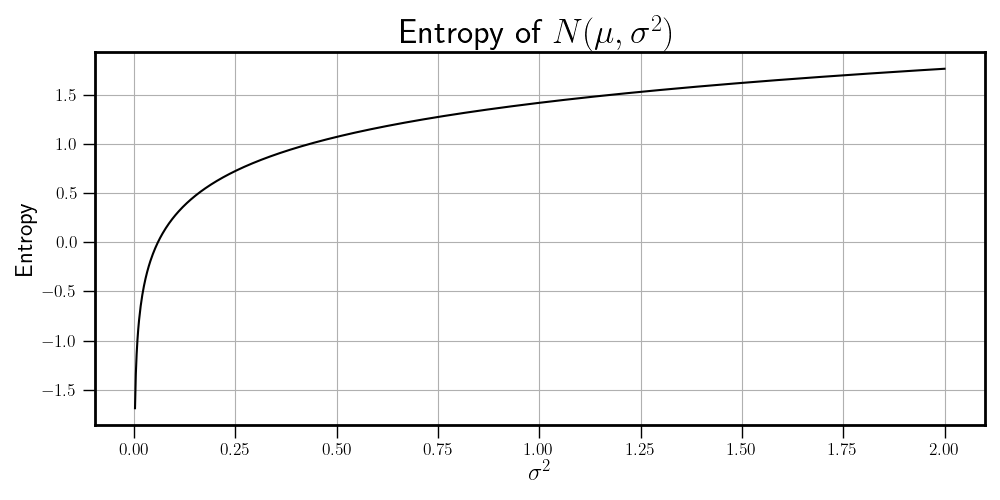
\includegraphics[width=\textwidth]{Figures/entropy_example.png}
    \end{minipage}%
    \begin{minipage}{.5\textwidth}
        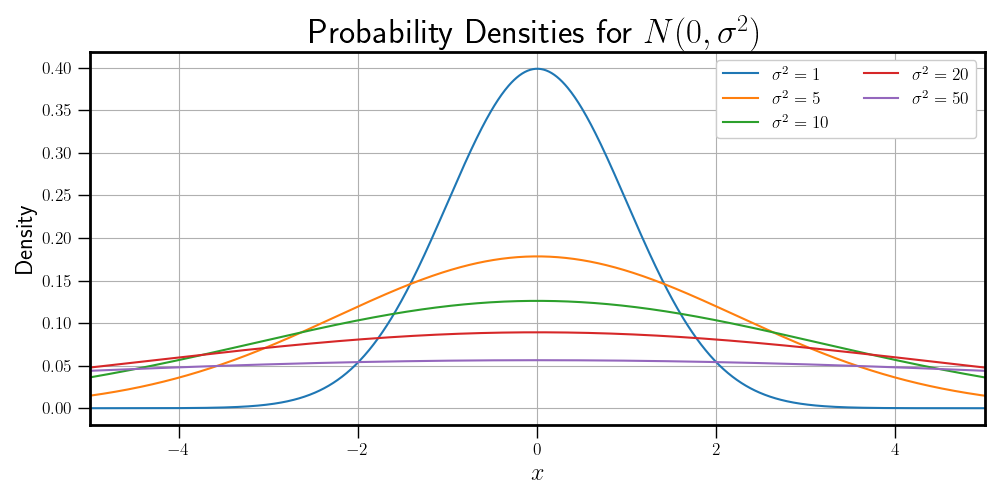
\includegraphics[width=\textwidth]{Figures/densities_example.png}
    \end{minipage}

    \caption{Entropy and density function change with respect to $\sigma^2$. The base 
    of the logarithm shown here is $e$, but the base itself is irrelevant due to the shared
    properties of all logarithms: that they increase monotonically and unbounded. As the 
    variance increases we see higher entropy in the left plot and a flattening of the 
    probability density in the right plot.}
    \label{fig:entropy example}
\end{figure}

\section{Basic Definitions}
The KL Divergence (KLD) is a statistical distance between a 
pair of probability distributions which measures how different a distribution $P$ is 
from a reference distribution $Q$. ``A simple interpretation of the 
divergence of $P$ from $Q$ is the expected excess surprise from using $Q$ as a model 
when the actual distribution is $P$.'' If $P$ and $Q$ are discrete distributions 
defined on the probability space $\mathcal{X}$, then the KLD of $P$ with 
respect to $Q$ is given by
\begin{equation}
    D_{KL}(P\ |\!|\ Q) = \sum_{x \in \mathcal{X}}P(x)\log\parens{P(x)/Q(x)} \label{eqn:discrete KLD}
\end{equation}
In other words, it is the expectation of the logarithmic difference between the 
probabilities $P$ and $Q$, where the expectation is taken using the probabilities 
$P$. As a ``distance'', the KLD is non-negative and 0 when $P = Q$ almost
everywhere. Unlike more standard metrics, it is not symmetric and does not satisfy 
the triangle equality. In order to deal with something that is, at least, symmetric 
we'll consider using the symmetric KL Divergence (SKLD) which is defined as 
\begin{equation}
    D_{SKL}(P, Q) = \frac{1}{2}\parens{D_{KL}(P\ |\!|\ Q) + D_{KL}(Q\ |\!|\ P)}
\end{equation}
Which is the average of the KLD for $P$ with respect to $Q$ and for $Q$
with respect to $P$. In our cases, we'll be dealing with a continuous random variable
with probability density functions $p$ and $q$, for which the corresponding KLD formula 
is
\begin{equation}
    D_{KL}(P\ |\!|\ Q) = \int_\mathcal{X} p(x)\log\parens{p(x)/q(x)}\ dx \label{eqn:continuous KLD}
\end{equation}
As an analogue of the discrete case, the same simple interpretations about
the formula apply. The reason we can consider this a ``distance'' is that the KLD 
is non-negative, $D_{KL}(P\ |\!|\ Q) \geq 0$, which is known as Gibbs 
inequality and only equals 0 when $P = Q$ almost everywhere. As such, the distance
between $P$ and $Q$ is 0 when they are the ``same'' distribution and some positive 
number if they differ. For example, consider the random variables $X_1 \sim 
\mathcal{N}(\mu_1, \sigma_1^2)$ and $X_2 \sim \mathcal{N}(\mu_2, \sigma_2^2)$ 
with corresponding density functions given by equation \ref{eqn:normal}; the divergence 
between the distributions is
\begin{equation}
    D_{KL}(p\ |\!|\ q) = \frac{1}{2}\parens{\ln\parens{\frac{\sigma_2^2}{\sigma_1^2}} + 
    \frac{\sigma_1^2}{\sigma_2^2} + \frac{(\mu_1 - \mu_2)^2}{\sigma_2^2} - 1}, \label{eqn:normal divergence}
\end{equation}
Letting $\mu_1 = \mu_2$, $\sigma_1^2 = 1$, and allowing $\sigma_2^2$ to vary, we can 
write 
\begin{equation}
    D_{KL}(p\ |\!|\ q) = \frac{1}{2}\parens{\ln\sigma_2^2 + 
    \frac{1}{\sigma_2^2} - 1}, \label{eqn:normal divergence2}
\end{equation}
\begin{figure}[ht]
    \centering
    \begin{minipage}{\textwidth}
        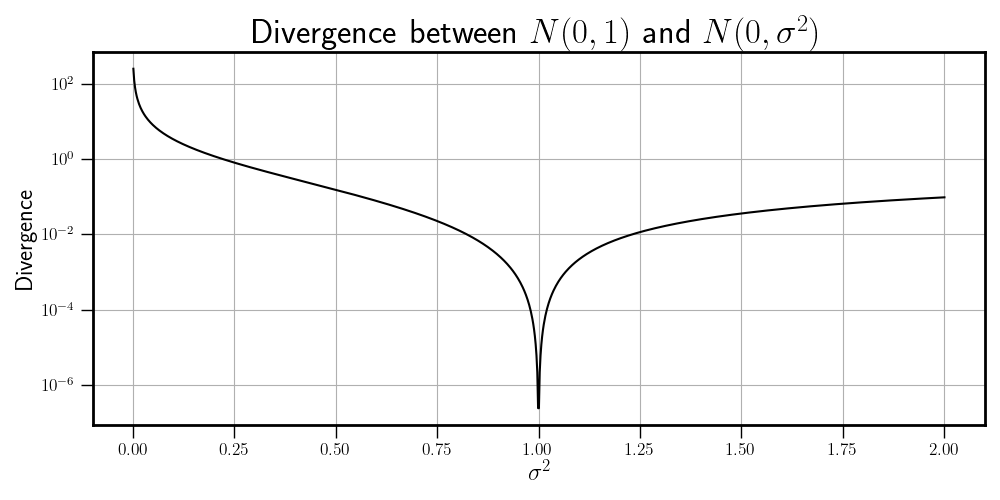
\includegraphics[width=\textwidth]{Figures/divergence_example.png}
    \end{minipage} 
    \caption{KL Divergence example with Normal distributions. As expected, the divergence 
    decreases to 0 as $\sigma^2 \to 1$ from either direction.}
    \label{fig:divergence example}
\end{figure}
Figure \ref{fig:divergence example} illustrates the KLD between the example normal distributions.

\section{How to build distributions (Non-parametric statistics)}
The question remains about how we obtain the probability distribution of the random 
variable that represents the evolution of each layer of an ML model from measured data. 
Many techniques exist, but we'll be using Kernel Density Estimation (KDE). The most 
basic idea behind KDE is using a different bin centering method and a smoothing factor, 
called a kernel, to approximate a probability density $f$ from measured data in the form 
of a histogram. This is accomplished with the \emph{kernel density estimator} for $f$
given by:
$$\hat{f}(x; K, h) = \frac{1}{nh}\sum_{i = 1}^n K\parens{\frac{x - x_i}{h}}$$
where $K$ is the chosen kernel, $h$ is what's called the bandwidth parameter, and 
$\{x_i\}_{i=1}^n$ is the data that generates our histogram. Per \cite{epanechnikov}, 
the choice of kernel does not provide much statistical significance; but the choice of 
the bandwidth parameter $h$ is very crucial for finding a density estimate that 
approximates the 
underlying density function appropriately. Choosing an optimal $h$ depends on 
the given data and the common method, Silverman's rule of thumb, works on the 
assumption that the density function of the data is unimodal and close to 
normal. For general data, on which no assumptions of normality are made, a more 
general method is found in the Improved Sheather-Jones algorithm (ISJ)\cite{botev}. 
The ISJ seeks to minimize the assymptotic mean integrated squared error (AMISE) of 
the estimator $\hat{f}$ with respect to $h$, which is given by 
\begin{equation}
    \text{AMISE}(\hat{f}) = \frac{h^2}{4}\norm{f''}^2 + \frac{1}{2n\sqrt{h\pi}}
\end{equation}
and depends on the unknown quantity $\norm{f''}$. The ISJ uses an iterative method 
based on the data and kernel function to approximate $\norm{f''}$ and arrive at 
the best bandwidth for the given data.


\section{Measuring entropy flow}
At each epoch $n$ of training for each layer $l$ in the encoder $\mathcal{E}$ and 
decoder $\mathcal{D}$ networks of the DLDMD algorithm, we generate an affliated matrix 
of weights ${\bf W}_{l,\mathcal{E}}^{(n)}$ and ${\bf W}_{l,\mathcal{D}}^{(n)}$, respectively.
Should any given training cause the machine to converge to a fixed state, then for each layer
we should have that
\begin{equation}
    {\bf W}_{l,\mathcal{E}}^{(n)}, {\bf W}_{l,\mathcal{D}}^{(n)} \to 
    {\bf W}_{l,\mathcal{E}}^{*}, {\bf W}_{l,\mathcal{D}}^{*} \text{ as }
    n \to \infty \label{eqn:weight convergence}
\end{equation}
Consequently, we can charaterize any set of weights via the formulas
\begin{equation}
    {\bf W}_{l,\mathcal{E}}^{(n)} = {\bf W}_{l,\mathcal{E}}^{*} + {\bf W}_{l,\mathcal{E}}^{(n),f},\
    {\bf W}_{l,\mathcal{D}}^{(n)} = {\bf W}_{l,\mathcal{D}}^{*} + {\bf W}_{l,\mathcal{D}}^{(n),f},
\end{equation}
where the fluctuation matrices ${\bf W}_{l,\mathcal{E}}^{(n),f}$ and 
${\bf W}_{l,\mathcal{D}}^{(n),f}$ are defined implicitly. These fluctuations are what we're 
most interested in studying. Using first-order differencing, we can study the affliated 
detrended matrices $\delta{\bf W}_{l,\mathcal{E}}^{(n)}$ where
\begin{align*}
    \delta{\bf W}_{l,\mathcal{E}}^{(n)} &= {\bf W}_{l,\mathcal{E}}^{(n+1)} - {\bf W}_{l,\mathcal{E}}^{(n)} \\
    &= {\bf W}_{l,\mathcal{E}}^{(n+1),f} - {\bf W}_{l,\mathcal{E}}^{(n),f}
\end{align*}
The definitions for the decoder weights are identical, and thus omitted. We can consider 
$\delta{\bf W}_{l,\mathcal{E}}^{(n)}$ to be the deviation from the steady state and with it 
in hand we flatten it's data and use KDE to generate an affliated empirical probability 
distribution $p_{l,\mathcal{E}}^{(n)}(w)$. With these distributions we know find the KLD 
between consecutive distributions to generate the following sequence: 
\begin{equation}
    D = \bracks{D_{KL}\parens{p_{l,\mathcal{E}}^{(n+1)} \Big|\!\Big| p_{l,\mathcal{E}}^{(n)}}}_{n=1}^{N_E - 2}
\end{equation}
which we can interpret to be the change in information between consecutive fluctuations from the 
steady state.

\section{Implementation Details}
The devil is in the details with respect to how this analysis is carried out and we will
go over the important ones here. After the training of each model for $N_E$ epochs, the 
data that we have to play with is 
\begin{equation}
    {\bf W}_\mathcal{E} = \bracks{{\bf W}_{l,\mathcal{E}}^{(n)}}_{n=1, l=1}^{N_E, N_l}, 
    {\bf W}_\mathcal{D} = \bracks{{\bf W}_{l,\mathcal{D}}^{(n)}}_{n=1, l=1}^{N_E, N_l}, 
\end{equation}
which are the sets of weights of the layers of the encoder and decoder. Note that both sub-networks 
have the same number of layers and only differ by the dimension of their inputs and outputs.
The following procedures are identical for both sets, so we'll only be referencing the encoder set
from here on out. For each layer $l$, the set of detrended matrices are computed
\begin{equation}
    \delta{\bf W}_{l, \mathcal{E}} = \bracks{{\bf W}_{l,\mathcal{E}}^{(n+1),f} - {\bf W}_{l,\mathcal{E}}^{(n),f}}_{n=1}^{N_E-1},
\end{equation}
these matrices are flattened and their entries are used as the data for KDE. The KDE implementation
used is that of KDEpy ({\bf https://pypi.org/project/KDEpy/}), which implements several 
algorithms for KDE in python including the bandwidth computation of ISJ. The kernel used is the Epanechnikov
kernel, defined as 
\begin{equation}
    K(x) = 
    \begin{cases}
        \frac{3(1-x^2)}{4}, & \abs{x} < 1 \\
        0, & \text{else}
    \end{cases},\label{eqn:epanechnikov}
\end{equation}
which is optimal in the mean square error sense. However, the choice of kernel is not a statistically 
significant one\cite{epanechnikov} and we choose this kernel for the convenience of it having finite 
support and non-vanishing first and second derivative on that support. The ISJ algorithm is used to 
determine the appropriate bandwidth for each set of data. These bandwidths are also being saved to 
see if the optimal bandwidth with respect to each data set might also contain some instructive 
information for quantification. From this, we obtain the set of density estimates for each detrended 
matrix
\begin{equation}
    p_{l,\mathcal{E}} = \text{KDE}(\delta{\bf W}_{l, \mathcal{E}}) = \bracks{p_{l,\mathcal{E}}^{(n)}(w)}_{n=1}^{N_E-1}
\end{equation}
where $w$ is the weight value itself and $p_{l,\mathcal{E}}(w)$ is the approximate density associated 
with that weight value. For the sake of our discretization of this data, we use 10001 linearly spaced 
points to represent the weights of each distribution from the smallest weight to the largest. The number 
of discrete points is also of some importance for the next step; given these density approximations, we 
can now compute what we're truly interested in: the relative entropy of consecutive densities and the 
associated change in information:
\begin{equation}
    D_l = \bracks{D_{SKL}\parens{p_{l,\mathcal{E}}^{(n+1)} \Big|\!\Big| p_{l,\mathcal{E}}^{(n)}}}_{n=1}^{N_E-2}
\end{equation}
Unlike in the first mention of entropy flow, we instead use the SKLD instead of the KLD. This consideration
simplifies our analysis by disregarding the asymmertric nature of KLD and consequences of this choice 
will be discussed in Chapter \ref{chap:discussion}. Given the discretized nature of the densities, we turn 
to numerical integration to compute the integral in Equation \ref{eqn:continuous KLD}. For the sake of an 
apples to apples comparison, we make the assumption that all densities have the same support
and use the 10001 discretized points with Simpson's rule for the integral approximation. Each set of these
divergences corresponds to a layer in the full network, and we can now use the divergences to characterize
how the information is changing with respect to the steady state. Figure \ref{fig:divergence of model example}
shows an example of the divergence over the whole training. 

We're interested in what these divergences tell 
us about information flow in the model's weights, and as such we seek a fitting of the data. Any overall trends
are more important to our analysis than lone data points, so to avoid transient behavior skewing any fittings
we ignore the first 20\% of the divergences computed. The values span several orders of magnitude, so a simple 
fitting would certainly fail and we instead attempt a linear fit on the base 10 logarithm of the data. This 
corresponds to an exponential fit in the original domain of the divergences with slope of the linear trend 
being the approximate growth/decay rate of the information flow from the machines steady state. The slope 
intercept is not so important for this reason, being only a constant that modifies the order of magnitude 
without changing the trens, so for the time being we ignore it. In the interest of trying to identify a 
classifier of good training, we then find the average and variance of the slopes of the linear fits of 
the layers' divergence data. The backbone of our results is to compare these averages for each latent 
dimension to the loss curves and phase portraits from the training for each dimension.

\begin{figure}[ht]
    \centering
    \begin{minipage}{\textwidth}
        \includegraphics[width=\textwidth]{"Z:/ML_models/DLDMD-newest/examples/van_der_pol/trained_models/van_der_pol_07_2022-07-17-1837/bandwidth_ISJ/div_plot_linear_enc_1"}
    \end{minipage}
    \caption{Example of divergences for layer Enc 1 of Van der Pol model with latent dimension 7 
    with linear fitting and confidence bands.}
    \label{fig:divergence of model example}
\end{figure}


\chapter{RESULTS}
\label{chap:results}
From experimentation by \cite{lago}, we know that some sets of hyperparameters yield good reconstruction
of the structure of the phase space of each of the dynamical systems in question and that some do not. For
the sake of testing our method of measuring information change, we elect to focus on changing only the 
lifting or latent dimension of the observables we wish to use for the DMD algorithm. After conducting 
multiple trainings with latent dimensions ranging from $N_O = 2$ to $N_O = 10$ for the Duffing and Van der 
Pol oscillators, the algorithm detailed in Chapter \ref{chap:KLD} was implemented. The initial hope of our 
analysis is the data points that our algorithm generates 
will show clear trends that will allow us to easily differentiate the optimal parameter choice for the 
model from suboptimal or even bad parameter choices. Given the model's task of learning an imbedding and 
find optimal observables in the latent space, we additionally surmised that we would see the most 
variability in the model in what we call the edge layers: Enc in, Enc out, Dec in and Dec out. The 
other layers in the model certaintly accomplish something as the model trains, but the dimension changes 
that help E-DMD along are accomplished at the edge layers, so we expect them to evolve differently than
the hidden layers. 

Though not explicitly
part of the algorithm, we'll examine how the bandwidths generated by the ISJ method might also give us 
insight into optimal parameter choice as well. As a surrogate of the bin size of the affliated histogram
of the data, it can give us an idea of how small a window each possible weight can exist in and examining
their evolution can give us an idea of how the shape of the empirical density is changing by epoch


\section{The Duffing Oscillator}
\label{section:duffing results}

\begin{figure}[!ht]
    \centering
    \begin{minipage}{\textwidth}
        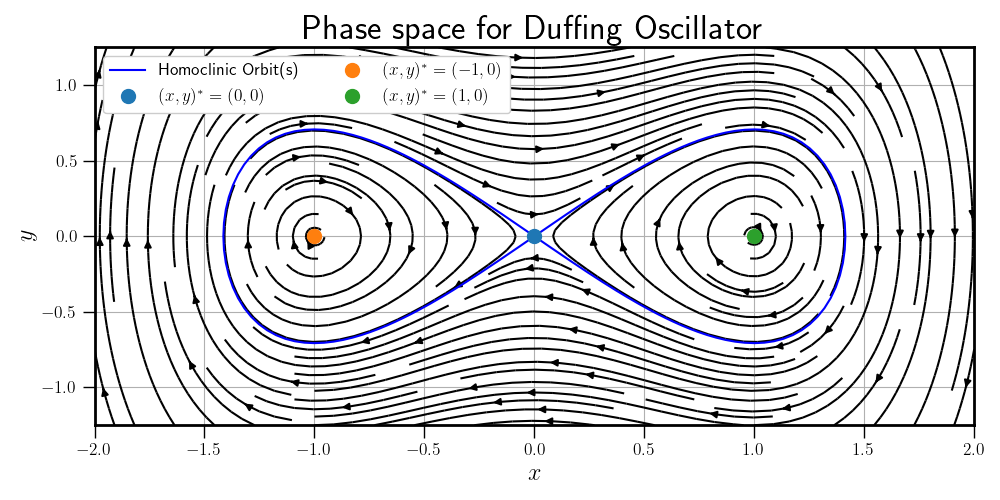
\includegraphics[width=\textwidth]{"Figures/duffing_phase_space.png"}
    \end{minipage}
    \caption{Duffing phase space.}
    \label{fig:duffing phase space}
\end{figure}

The Duffing oscillator is a non-linear second-order differential equation used to model 
certain damped and driven oscillators, whose general form is given by
\begin{equation}
    \ddot{x} + \delta\dot{x} + \alpha x + \beta x^3 = \gamma\cos(\omega t)
\end{equation}
There are many sets of coefficients for which many types of behvior are exhibited by the
system; but for our purposes we'll only consider the following configuration:
\begin{equation}
    \ddot{x} - x + x^3 = 0
\end{equation}
which when turned into a system of first-order equations by introducing $y = \dot{x}$ is
\begin{equation}
    \begin{cases}
        & \dot{x} = y \\
        & \dot{y} = x - x^3  
    \end{cases}
\end{equation}

\begin{table}[!ht]
    \centering
    \begin{minipage}{.7\textwidth}
        \caption{Hyperparamters of the DLDMD algorithm held constant for each training run on Duffing.}
        \label{table:duffing params}
        \begin{tabularx}{\textwidth}{|>{\centering\arraybackslash}X|>{\centering\arraybackslash}X|} \hline% {\columnwidth}{|@{\extracolsep{\stretch{1}}}*{1}{c}@{}|@{\extracolsep{\stretch{1}}}*{1}{c}@{}|}\hline
            Hyperparameter & Value \\ \hline \hline
            Initial Conditions & 15000 \\ \hline
            Training proportion & $66.66\%$ \\ \hline
            Validation proportion & $19.98\%$ \\ \hline
            Testing proportion & $13.36\%$ \\ \hline
            Optimizer & Adam \\ \hline
            $t_0$ & 0 \\ \hline
            $\Delta t$ & 0.05 \\ \hline
            $t_f$ & 20 \\ \hline
            $N_E$ & 1000 \\ \hline
            Enc/Dec layers & 3 \\ \hline
            Enc/Dec hidden activation & ELU \\ \hline
            Enc/Dec output activation & identity \\ \hline
            % Dec/Dec layers & 3 \\ \hline
            % Dec/Dec hidden activation & elu \\ \hline
            % Dec/Dec output activation & identity \\ \hline
            Neurons/layer & 128 \\ \hline
            Weight initializer & $\mathcal{N}(0, .1, 2)$ \\ \hline
            Bias Initializer & 0 \\ \hline
            Learning Rate & $10^{-3}$ \\ \hline
            $a_1,\ a_2,\ a_3$ & 1 \\ \hline
            $a_4$ & $10^{-14}$ \\ \hline
        \end{tabularx}
    \end{minipage}
\end{table}

The interesting attributes of this system are that it has 3 fixed points, 2 of which are non-linear 
centers with the third being a saddle point with homoclinic connections that encompass the other 2 fixed 
points. Figure \ref{fig:duffing phase space} shows a graphical representation of the phase space of our 
Duffing oscillator. The homoclinic connection itself provides an interesting challenge topologically in 
that it divides the phase space into distinct regions that affect the end behavior of the system depending
on the initial condition. Table \ref{table:duffing params} describes the hyperparameters used for the 
Duffing Oscillator that were left unchanged for each run; note that the distribution given as 
$\mathcal{N}(\mu, \sigma^2, n)$ is the truncated normal distribution, which is a normal distribution
in which all values drawn that are more than $n$ standard deviations from the mean are discarded. 

A few notes on the trainings themselves are worth mentioning here. No learning rate scheduling is used,
so the learning rate with the Adam optimizer is held constant for all epochs. The activation function
Exponential Linear Unit (ELU) is used instead of the more standard Rectified Linear Unit (ReLU) due an 
error that occurs in the numerics of DLDMD for latent dimension choices greater than 3. ELU is a 
parameterized activation function whose definition is given in Table \ref{table:elu vs relu} and is closely
related to ReLU; in fact, if the parameter $\alpha$ is set to 0 then ELU and ReLU are identical. For the
sake of having similar performance for ELU with respect to ReLU, we choose $\alpha = .01$. For reasons still 
under investigation, the RELU activation function causes the Singular Value Decomposition to fail if the 
latent dimension is 3 or greater and the algorithm subsequently ends with an error. After experimentation, 
it was found that using ELU instead circumvents this problem without significantly affecting model training.
As a final note, the training for this model (and Van der Pol) across all latent dimensions was done on the 
same data set with the same subsets chosen to be the training, test, and validation data. We do this to
reduce the number of variables down to the latent dimension alone.
\begin{figure}[!ht]
    \centering
    \begin{minipage}{\textwidth}
        \includegraphics[width=\textwidth]{"Z:/ML_models/DLDMD-newest/examples/duffing/slope_linear_fit.png"} 
    \end{minipage}%
    \caption{Duffing average slopes with standard deviations.}
    \label{fig:duffing average slopes}
\end{figure}

Having established this, we'll consider the results of our analysis.
Figure \ref{fig:duffing average slopes} shows the average of the slopes of the linear fits across 
all layers for each epoch.  What we can see plainly is that for latent dimensions 2 through 5, the average
slope is small in magnitude with a small to medium standard deviation relative to the scale with
latent dimension 6 showing not only a much larger average slope, but as also much more variance. We may 
contrast this with the losses in Figure \ref{fig:duffing losses} for each latent dimension, which seems 
to show that latent dimension 5 should be the optimal choice with all other choices being more or less 
equivalent. This does not match the results of the phase space representation, which show roughly that 
dimension 3 is best. 
If we examine Figure \ref{fig:duffing average bandwidth}, which shows the average bandwidth from the ISJ
algorithm across all layer for a given latent dimension per epoch, we can see that 3 has a slightly
different trend and separates cleanly from each of the other choices. While this behavior tracks with our 
understanding that this dimension is best and should be easily differentiated from the rest, it is 
inconsistent the fact that the other bandwidth curves are banded together but don't have much in common
with respect to Figures \ref{fig:duffing average slopes} and \ref{fig:duffing losses}
for both the fitted slopes and loss curves.


\begin{figure}[!ht]
    \centering
    \begin{minipage}{\textwidth}
        \includegraphics[width=\textwidth]{"Z:/ML_models/DLDMD-newest/examples/duffing/loss_plots.png"} 
    \end{minipage}%
    \caption{Duffing loss plots, smoothed to accentuate trends.}
    \label{fig:duffing losses}
\end{figure}

\begin{figure}[!ht]
    \centering
    \begin{minipage}{\textwidth}
        \includegraphics[width=\textwidth]{"Z:/ML_models/DLDMD-newest/examples/duffing/bandwidth_averages_plot.png"} 
    \end{minipage} 
    \caption{Duffing Average bandwidth.}
    \label{fig:duffing average bandwidth}
\end{figure}

For a more granular view of the individual fittings for each layer of the model, we have Figures 
\ref{fig:duffing slopes all layers} and \ref{fig:duffing linear fits all layers}. Much to our 
expectation, the plots for the edge layers have slightly different behavior than for the hidden layers;
generally, the linear trends have a smaller slope and y-intercept further from 0. We can interpret this 
as being indicative of having an information change trend that is further from the theoretical steady-state
than for the other layers of the model. We've come to associate this with the kind of expressivity that is
desireable for ML models to have in that they are able to cope with the kind of variability that real world 
data could exhibit. The ultimate conclusion we're able to draw is that DLDMD seems to adequately train and 
predict future states of Duffing for latent dimensions smaller than 6.

\begin{figure}[!htbp]
    \centering
    \begin{minipage}{.5\textwidth}
        \includegraphics[width=\textwidth]{"Z:/ML_models/DLDMD-newest/examples/duffing/slope_linear_fit_enc_in.png"} 
        \includegraphics[width=\textwidth]{"Z:/ML_models/DLDMD-newest/examples/duffing/slope_linear_fit_enc_0.png"} 
        \includegraphics[width=\textwidth]{"Z:/ML_models/DLDMD-newest/examples/duffing/slope_linear_fit_enc_1.png"} 
        \includegraphics[width=\textwidth]{"Z:/ML_models/DLDMD-newest/examples/duffing/slope_linear_fit_enc_2.png"} 
        \includegraphics[width=\textwidth]{"Z:/ML_models/DLDMD-newest/examples/duffing/slope_linear_fit_enc_out.png"} 
    \end{minipage}%
    \begin{minipage}{.5\textwidth}
        \includegraphics[width=\textwidth]{"Z:/ML_models/DLDMD-newest/examples/duffing/slope_linear_fit_dec_in.png"} 
        \includegraphics[width=\textwidth]{"Z:/ML_models/DLDMD-newest/examples/duffing/slope_linear_fit_dec_0.png"} 
        \includegraphics[width=\textwidth]{"Z:/ML_models/DLDMD-newest/examples/duffing/slope_linear_fit_dec_1.png"} 
        \includegraphics[width=\textwidth]{"Z:/ML_models/DLDMD-newest/examples/duffing/slope_linear_fit_dec_2.png"} 
        \includegraphics[width=\textwidth]{"Z:/ML_models/DLDMD-newest/examples/duffing/slope_linear_fit_dec_out.png"} 
    \end{minipage}
    \caption{Duffing slope linear fits by layer.}
    \label{fig:duffing slopes all layers}
\end{figure}

\begin{figure}[!htbp]
    \centering
    \begin{minipage}{.5\textwidth}
        \includegraphics[width=\textwidth]{"Z:/ML_models/DLDMD-newest/examples/duffing/div_plot_linear_enc_in.png"} 
        \includegraphics[width=\textwidth]{"Z:/ML_models/DLDMD-newest/examples/duffing/div_plot_linear_enc_0.png"} 
        \includegraphics[width=\textwidth]{"Z:/ML_models/DLDMD-newest/examples/duffing/div_plot_linear_enc_1.png"} 
        \includegraphics[width=\textwidth]{"Z:/ML_models/DLDMD-newest/examples/duffing/div_plot_linear_enc_2.png"} 
        \includegraphics[width=\textwidth]{"Z:/ML_models/DLDMD-newest/examples/duffing/div_plot_linear_enc_out.png"} 
    \end{minipage}%
    \begin{minipage}{.5\textwidth}
        \includegraphics[width=\textwidth]{"Z:/ML_models/DLDMD-newest/examples/duffing/div_plot_linear_dec_in.png"} 
        \includegraphics[width=\textwidth]{"Z:/ML_models/DLDMD-newest/examples/duffing/div_plot_linear_dec_0.png"} 
        \includegraphics[width=\textwidth]{"Z:/ML_models/DLDMD-newest/examples/duffing/div_plot_linear_dec_1.png"} 
        \includegraphics[width=\textwidth]{"Z:/ML_models/DLDMD-newest/examples/duffing/div_plot_linear_dec_2.png"} 
        \includegraphics[width=\textwidth]{"Z:/ML_models/DLDMD-newest/examples/duffing/div_plot_linear_dec_out.png"} 
    \end{minipage}
    \caption{Duffing slope linear fits by layer.}
    \label{fig:duffing linear fits all layers}
\end{figure}

\begin{figure}[!htbp]
    \centering
    \begin{minipage}{.5\textwidth}
        \includegraphics[width=\textwidth]{"Z:/ML_models/DLDMD-newest/examples/duffing/trajectories_00.png"} 
        \includegraphics[width=\textwidth]{"Z:/ML_models/DLDMD-newest/examples/duffing/trajectories_03.png"} 
        \includegraphics[width=\textwidth]{"Z:/ML_models/DLDMD-newest/examples/duffing/trajectories_05.png"} 
        \includegraphics[width=\textwidth]{"Z:/ML_models/DLDMD-newest/examples/duffing/trajectories_00.png"} 
        \includegraphics[width=\textwidth]{"Z:/ML_models/DLDMD-newest/examples/duffing/trajectories_00.png"} 
    \end{minipage}%
    \begin{minipage}{.5\textwidth}
        \includegraphics[width=\textwidth]{"Z:/ML_models/DLDMD-newest/examples/duffing/trajectories_02.png"} 
        \includegraphics[width=\textwidth]{"Z:/ML_models/DLDMD-newest/examples/duffing/trajectories_04.png"} 
        \includegraphics[width=\textwidth]{"Z:/ML_models/DLDMD-newest/examples/duffing/trajectories_06.png"} 
        \includegraphics[width=\textwidth]{"Z:/ML_models/DLDMD-newest/examples/duffing/trajectories_00.png"} 
        \includegraphics[width=\textwidth]{"Z:/ML_models/DLDMD-newest/examples/duffing/trajectories_00.png"} 
    \end{minipage}
    \caption{Duffing DLDMD results.}
    \label{fig:duffing DLDMD results}
\end{figure}

\begin{table}[!htb]
    \centering
    \begin{minipage}{\textwidth}
        \caption{ReLU activation function vs ELU activation function.}
        \label{table:elu vs relu}
        \begin{tabularx}{\textwidth}{|>{\centering\arraybackslash}X|>{\centering\arraybackslash}X|} \hline% {\columnwidth}{|@{\extracolsep{\stretch{1}}}*{1}{c}@{}|@{\extracolsep{\stretch{1}}}*{1}{c}@{}|}\hline
            ReLU & ELU \\ \hline \hline
            $\sigma(x) = \begin{cases}
                x, & x > 0 \\
                0, & \text{else}
            \end{cases}$ & 
            $\sigma(x; \alpha) = \begin{cases}
                x, & x > 0 \\
                \alpha(e^x - 1), & \text{else}
            \end{cases}$ \\ \hline
        \end{tabularx}
    \end{minipage}
\end{table}

\section{The Van der Pol Oscillator}
\label{section:van der pol results}

\begin{figure}[ht]
    \centering
    \begin{minipage}{\textwidth}
        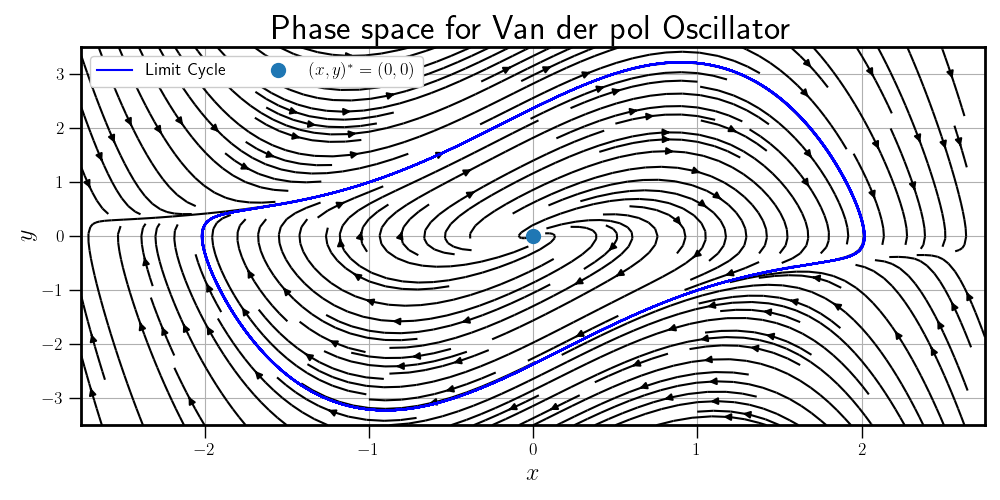
\includegraphics[width=\textwidth]{"Figures/van_der_pol_phase_space.png"} 
    \end{minipage}
    \caption{Van der Pol phase space.}
    \label{fig:van der pol phase space}
\end{figure}

The Van der Pol oscillator is a non-conservative oscillator with non-linear damping, and models a more 
specific kind of circuit than Duffing does. It's general form is given by 
\begin{equation}
    \ddot{x} - \mu(1 - x^2)\dot{x} + x = 0
\end{equation}
Much like Duffing, varying $\mu$ can give different and interesting phase space dynamics. For our
purposes we will fix it to $\mu = 1.5$. With this, the equivalent system of first order equations
is 
\begin{equation}
    \begin{cases}
        & \dot{x} = y \\
        & \dot{y} = 1.5(1 - x^2)y - x  
    \end{cases}
\end{equation}

\begin{figure}[ht]
    \centering
    \begin{minipage}{\textwidth}
        \includegraphics[width=\textwidth]{"Z:/ML_models/DLDMD-newest/examples/van_der_pol/slope_linear_fit.png"} 
    \end{minipage}
    \caption{Van der Pol average slopes with standard deviations.}
    \label{fig:van der pol average slopes}
\end{figure}

Again, by introducing $y = \dot{x}$. Unlike Duffing, this system has a single unstable fixed point
at the origin and all nontrivial orbits are attracted to a limit cycle that surrounds the origin. 
Figure \ref{fig:van der pol phase space} shows a graphical representation of the phase space of our 
Van der Pol oscillator. Much like Duffing, we do have a curve that separates the phase space into 
regions of different behavior in the limit cycle; but since all orbits approach the limit cycle there
should be much variability with respect to initial conditions. We would expect training on this system 
to be better overall due to the fact that all trajectories are essentially going to same place unlike
the more complex behavior of Duffing. The hyperparameters for the Van der Pol
training are identical to those of Duffing with the exception of the activation function; which is, 
as mentioned in Section \ref{section:duffing results}, changed to ReLU. This difference 
is minor enough that a Van der Pol hyperparameters table is omitted.

\begin{figure}[ht]
    \centering
    \begin{minipage}{\textwidth}
        \includegraphics[width=\textwidth]{"Z:/ML_models/DLDMD-newest/examples/van_der_pol/loss_plots.png"} 
    \end{minipage}
    \caption{Van der Pol loss plots, smoothed to accentuate trend.}
    \label{fig:van der pol losses}
\end{figure}

Figure \ref{fig:van der pol average slopes}, shows the average and standard deviation of the slopes for 
the Van der Pol training per latent dimension choice. Relative to Figure \ref{fig:duffing average slopes}
for Duffing, we have larger average slopes and more variety with respect to the standard deviations for 
each dimension. Based on the phase plane results, we should expect 8 to correspond to the best training 
so it seems that a small in magnitude slope is indicative of good training and this in consistent for
some of the loss curves in Figure \ref{fig:van der pol losses}. The slope of 5 is essentially 0 and 
we that it has a loss curve almost indistinguishable from that of 8; and we can make a similar observation
about 7 as well. However, 10 also has a small slope but the loss curve is markedly different from the 
optimal choices and seems to match that of 3 which has a very large slope comparitively. One quality
the optimal trainings seem to have in common is that they have smaller standard deviations than the 
trainings with worse loss curves. 

\begin{figure}[ht]
    \centering
    \begin{minipage}{\textwidth}
        \includegraphics[width=\textwidth]{"Z:/ML_models/DLDMD-newest/examples/van_der_pol/bandwidth_averages_plot.png"} 
    \end{minipage} 
    \caption{Van der Pol Average bandwidth.}
\end{figure}



\begin{figure}[h!p]
    \centering
    \begin{minipage}{.5\textwidth}
        \includegraphics[width=\textwidth]{"Z:/ML_models/DLDMD-newest/examples/van_der_pol/slope_linear_fit_enc_in.png"} 
        \includegraphics[width=\textwidth]{"Z:/ML_models/DLDMD-newest/examples/van_der_pol/slope_linear_fit_enc_0.png"} 
        \includegraphics[width=\textwidth]{"Z:/ML_models/DLDMD-newest/examples/van_der_pol/slope_linear_fit_enc_1.png"} 
        \includegraphics[width=\textwidth]{"Z:/ML_models/DLDMD-newest/examples/van_der_pol/slope_linear_fit_enc_2.png"} 
        \includegraphics[width=\textwidth]{"Z:/ML_models/DLDMD-newest/examples/van_der_pol/slope_linear_fit_enc_out.png"} 
    \end{minipage}%
    \begin{minipage}{.5\textwidth}
        \includegraphics[width=\textwidth]{"Z:/ML_models/DLDMD-newest/examples/van_der_pol/slope_linear_fit_dec_in.png"} 
        \includegraphics[width=\textwidth]{"Z:/ML_models/DLDMD-newest/examples/van_der_pol/slope_linear_fit_dec_0.png"} 
        \includegraphics[width=\textwidth]{"Z:/ML_models/DLDMD-newest/examples/van_der_pol/slope_linear_fit_dec_1.png"} 
        \includegraphics[width=\textwidth]{"Z:/ML_models/DLDMD-newest/examples/van_der_pol/slope_linear_fit_dec_2.png"} 
        \includegraphics[width=\textwidth]{"Z:/ML_models/DLDMD-newest/examples/van_der_pol/slope_linear_fit_dec_out.png"} 
    \end{minipage}
    \caption{Van der Pol slope linear fits by layer.}
    \label{fig:van der pol slopes all layers}
\end{figure}

\begin{figure}[h!p]
    \centering
    \begin{minipage}{.5\textwidth}
        \includegraphics[width=\textwidth]{"Z:/ML_models/DLDMD-newest/examples/van_der_pol/div_plot_linear_enc_in.png"} 
        \includegraphics[width=\textwidth]{"Z:/ML_models/DLDMD-newest/examples/van_der_pol/div_plot_linear_enc_0.png"} 
        \includegraphics[width=\textwidth]{"Z:/ML_models/DLDMD-newest/examples/van_der_pol/div_plot_linear_enc_1.png"} 
        \includegraphics[width=\textwidth]{"Z:/ML_models/DLDMD-newest/examples/van_der_pol/div_plot_linear_enc_2.png"} 
        \includegraphics[width=\textwidth]{"Z:/ML_models/DLDMD-newest/examples/van_der_pol/div_plot_linear_enc_out.png"} 
    \end{minipage}%
    \begin{minipage}{.5\textwidth}
        \includegraphics[width=\textwidth]{"Z:/ML_models/DLDMD-newest/examples/van_der_pol/div_plot_linear_dec_in.png"} 
        \includegraphics[width=\textwidth]{"Z:/ML_models/DLDMD-newest/examples/van_der_pol/div_plot_linear_dec_0.png"} 
        \includegraphics[width=\textwidth]{"Z:/ML_models/DLDMD-newest/examples/van_der_pol/div_plot_linear_dec_1.png"} 
        \includegraphics[width=\textwidth]{"Z:/ML_models/DLDMD-newest/examples/van_der_pol/div_plot_linear_dec_2.png"} 
        \includegraphics[width=\textwidth]{"Z:/ML_models/DLDMD-newest/examples/van_der_pol/div_plot_linear_dec_out.png"} 
    \end{minipage}
    \caption{Van der Pol slope linear fits by layer.}
    \label{fig:van der pol linear fits all layers}
\end{figure}

\begin{figure}[!htbp]
    \centering
    \begin{minipage}{.5\textwidth}
        \includegraphics[width=\textwidth]{"Z:/ML_models/DLDMD-newest/examples/van_der_pol/trajectories_00.png"} 
        \includegraphics[width=\textwidth]{"Z:/ML_models/DLDMD-newest/examples/van_der_pol/trajectories_03.png"} 
        \includegraphics[width=\textwidth]{"Z:/ML_models/DLDMD-newest/examples/van_der_pol/trajectories_05.png"} 
        \includegraphics[width=\textwidth]{"Z:/ML_models/DLDMD-newest/examples/van_der_pol/trajectories_07.png"} 
        \includegraphics[width=\textwidth]{"Z:/ML_models/DLDMD-newest/examples/van_der_pol/trajectories_09.png"} 
    \end{minipage}%
    \begin{minipage}{.5\textwidth}
        \includegraphics[width=\textwidth]{"Z:/ML_models/DLDMD-newest/examples/van_der_pol/trajectories_02.png"} 
        \includegraphics[width=\textwidth]{"Z:/ML_models/DLDMD-newest/examples/van_der_pol/trajectories_04.png"} 
        \includegraphics[width=\textwidth]{"Z:/ML_models/DLDMD-newest/examples/van_der_pol/trajectories_06.png"} 
        \includegraphics[width=\textwidth]{"Z:/ML_models/DLDMD-newest/examples/van_der_pol/trajectories_08.png"} 
        \includegraphics[width=\textwidth]{"Z:/ML_models/DLDMD-newest/examples/van_der_pol/trajectories_00.png"} 
    \end{minipage}
    \caption{Van der Pol DLDMD results.}
    \label{fig:van der pol DLDMD results}
\end{figure}

\chapter{DISCUSSION}
\label{chap:discussion}

While we believe that we've struck upon some useful results with respect to finding different behavior
and trends in some of the different values we've computed, it must be made clear that some assumptions
were made on our part that might not have been valid ones to makes given what we've learned since the 
outset. Some of which is detailed in the coming sections. Perhaps the biggest assumption made is that 
we have sets of optimal parameters at all for the DLDMD algorithm. There hasn't been much study into this 
algorithm yet, and the only measure of it's validity is given by \cite{lago} in their results and our 
replications which admittedly rely on the ``eye-ball'' metric. Predicting future states in multidimensional
nonlinear dynamical systems from time-series data is very tricky and it's difficult to quantify accuracy 
or whether key phase space features are respected in the predictions. Dealing with separatrices and 
the concentric centers, the prediction results, and the activation function issues of Duffing in 
particular casts some doubt on the parameters we have taken to be optimal. 

% Our results are also quite 
% idealized due to the perfect data from numerical integration that DLDMD uses 

\section{Non-unitary densities}
When creating the empirical densities in Chapter \ref{chap:results}, often we end up deriving 
density functions that don't exhibit a core property of density functions: The sum of their 
probabilities does not integrate to 1. KDE was doubtless designed for less pathological data than 
the kind we seem to be extracting from the weight matrices of the model. This perhaps conflicts with the 
assumption that we should be able to extract a density from the weight matrices at all. After some 
investigation, we've come to realize that the this is a consequence of the bandwidth use in KDE. 
For our density estimation, we made no assumptions about the shape or modality of the data and so 
the existing literature led us to using the ISJ to find an optimal bandwidth for each probability
density. The resulting densities are full of narrow peak and wide troughs, reminiscent of Dirac's comb;
which explains why the numerical integration schemes that are being used aren't giving us the areas we
expect. The bandwidths due to ISJ we're on the order of $10^{-6}$ and we found that using larger 
bandwidths led to overall smoother densities that we were able to numerically verify have approximately 
unitary area. The varying shapes based on bandwidth are another indicator of the inherent tradeoff 
between bias and variance in any model.

We have no reason to believe that there is anything at all wrong with the software package
being used for KDE and instead postulate that a more sophisticated scheme of integration, one that doesn't
rely as much on smooth data, is needed for the optimal bandwidth parameter. One silver-lining we can
deduce from this is that the apparent failure of boiler plate numerical integration can give us an idea
of how much variance a given derived density has and we can use that make other inferences about 
the model itself.

% Figure BLAH shows histograms of the numerically 
% computed areas of the densities yielded by KDE. Peaks are visible near 1 , but the spread around this average is not insignificant. 

% \begin{figure}[h!]
    % \centering
    % \begin{minipage}{\textwidth}
        % \includegraphics[width=\textwidth]{"Z:/ML_models/DLDMD-newest/examples/area_devs.png"} 
    % \end{minipage}%
    % \caption{Histograms of computed areas from KDE.}
    % \label{fig:area deviance}
% \end{figure}


\section{Statistical issues with edge layers}
The weight matrices are used in the model for linear transformations; the hidden layers 
have approximately $D^2$ entries while the edge layers 
have about $D\cdot d$ entries, where $D$ is the number of neurons in the layer and $d$ is the number 
of physical dimensions of the systems or the latent dimension. In either case, $d <\!\!< D$ so from a 
statistical standpoint the edge layers don't have as much data for the analysis. As we've elaborated on 
in Chapter \ref{chap:results}, we do notice marginally different behavior in the results for the edge 
layers than we do for the hidden layers and it's as of yet unclear whether this is evidence of the 
validity of our hypothesis or a consequence of having less data to fully characterize their evolution. 
For the range of latent dimensions we ran the model with, the hidden layers have approximately 16000 
data points and the edge layers can have as few as 258 data points or as many 1161 data points. This
spread alone leads to a belief that the higher latent dimensions should yield better results because
there are more trainable parameters and it is consistent with the expectation that more observables 
leads to an improved E-DMD in the lifted coordinates. It is, however, not consistent with all of the
results from DLDMD or the analysis in this thesis.

\section{Future work}
In the interest of future exploration of the ideas in this thesis, another ML model that would be 
excellent to examine would be a classifier of some kind. Such a problem would also allow us to use 
alternative metrics such as model accuracy (which is much easier to quantify than the for the dynamical 
systems we investigate) along with our analysis to get a better idea of the limits of this discovery of 
good training through the frame of information change. Such classifiers are all over the modern literature 
of ML and would have great interest in a method for determining good training during training would be of 
immense utility. Naturally, image processing applications of ML would be worth looking at through this 
lense considering how much more complex images are as inputs and that most applications implicitly
involve examining fine details with respect to the amount of information the image contains. It would
also provide an opportunity to experiment with NN architectures other than the Sequential model 
of DLDMD. 

Change in information content might also be a meaningful consideration for unsupervised training in 
that have another way to quantify if the model is arriving at a configuration that accomplishes the 
given task or not. 